\documentclass[12pt]{article}
\usepackage[margin = 2.5cm]{geometry}
\usepackage[utf8]{inputenc}
\usepackage[english]{babel}
\usepackage{amsmath}
\usepackage{graphicx}
\usepackage[T1]{fontenc}
\usepackage[natbibapa]{apacite}
\usepackage{hyperref}
\setcitestyle{notesep={:}}
\setcitestyle{maxcitenames=2}
\usepackage{booktabs, caption, longtable}
\usepackage{tabularx}
\usepackage{adjustbox}
\usepackage{pdfpages}
\usepackage{tabularray}
\usepackage{fancyhdr}
\usepackage{float}
\usepackage{subcaption}
\usepackage{nameref}

\usepackage{tikz}
\usetikzlibrary{calc}
\newcommand\HRule{\rule{\textwidth}{1pt}}

% line spacing
\linespread{1.5}

\begin{document}

\renewcommand{\refname}{Bibliography}

\begin{titlepage}

\begin{center}

% Upper part of the page
\textsc{\LARGE Universiteit Utrecht}\\[2.5cm]

\textsc{\Large Methodology \& Statistics for the Behavioural, Biomedical and Social Sciences}\\[1cm]
\textsc{\large Internship Report}\\[1cm]
% Title
\HRule \\[0.4cm]
{ \LARGE \bfseries Bayesian Evidence Synthesis: Aggregating evidence from partially overlapping hypotheses}\\[0.4cm]

\HRule \\[4cm]
\begin{minipage}{0.45\textwidth}
\begin{flushleft} \large
\emph{Author:}\\
Florian \textsc{Metwaly} \\
Student-Nr.: 0778265
\end{flushleft}
\end{minipage}
\begin{minipage}{0.45\textwidth}
\begin{flushright} \large
\emph{Supervisor:} \\
Irene \textsc{Klugist} \\
Duco \textsc{Veen} \\
Alfons \textsc{Edmar}
\end{flushright}
\end{minipage}

\vfill

% Bottom of the page
{\large \today} \\

\end{center}

\end{titlepage}

\tableofcontents
\newpage

\section{Introduction}
Common practice in research is to conduct meta-analyses, which aggregate evidence over multiple studies at the level of effect sizes, to draw more reliable and generalizable conclusions about a particular phenomenon. By combining the results of several studies, meta-analyses increase statistical power and reduce the uncertainty associated with individual studies that may have small sample sizes or inconsistent results. But, this is only possible if multiple studies are conceptual replications of each other. Bayesian Evidence Synthesis (BES) is an alternative for meta-analyses, which aggregates evidence on the level of the Bayes Factor (BF). As has been shown, BES can reliably aggregate the evidence over multiple studies with diverse study set-ups, as long as the underlying hypotheses represent the same underlying effect. \citet{kevenaar_bayesian_2021} used BES to aggregate the evidence over multiple studies, in which each study only contained information about part of an overarching hypothesis, while all studies together did cover the full range of the overarching hypothesis. This application of Bayesian Evidence Synthesis deems clear practical relevance, but the concept has yet to be proven. Therefore, this internship tries to answer the question: Is the synthesis of BFs from studies that evaluate only parts of the overarching hypothesis a good measure of joint support for the overarching hypothesis?

\section{Bayesian Evidence Synthesis}
The Bayes Factor quantifies the evidence for or against an informative hypothesis relative to either one other hypothesis or a set of hypotheses \citep{hoijtink_tutorial_2019}. The Bayes Factor is calculated by taking the ratio of the marginal likelihoods $m_1$ and $m_2$ of two hypotheses $H_1$ and $H_2$ \citep{chib_marginal_1995, kass_bayes_1995}
\begin{equation}
    BF_{1,2} = \frac{m_1}{m_2} = \frac{P(D|H_1)}{P(D|H_2)}.
\end{equation}
By reflecting the ratio of evidence for the different hypotheses, the $BF_{1,2}$ is interpreted as the amount of evidence for $H_1$ over $H_2$. An $BF_{1,2}$ of 10 therefore is interpreted as ten times the amount of evidence for $H_1$ over $H_2$. \\
There are different alternative hypotheses that can be used in a Bayesian Hypothesis Testing framework. Common choices include the complement hypothesis, the null hypothesis or the unconstrained hypothesis. In this report, the unconstrained hypothesis is further chosen as alternative hypothesis. The unconstrained hypothesis $H_u$ imposes no constraints and therefore allows the parameters to vary freely, without any specific restrictions or predefined values. Testing a hypothesis $H_1$ against the unconstrained hypothesis $H_u$ simplifies the calculation of the Bayes Factor to 
\begin{equation}
    BF_{1u} = \frac{m_1}{m_u} = \frac{f_1}{c_1}
\end{equation}
with $f_1$ being the fit and $c_1$ the complexity of $H_1$, as shown in \citet{klugkist_inequality_2005}. The fit $f_1$ is the proportion of the unconstrained posterior distribution that is in agreement with $H_1$, while the complexity $c_1$ is the proportion of the unconstrained prior distribution that is in agreement with $H_1$ \citep{hoijtink_informative_2011}. By using the Bayes Factor for hypothesis testing, as alternative to null hypothesis significance testing (NHST), one is able to test different informative hypotheses against each other. Further, as the Bayes Factor quantifies the support for a hypothesis, this method allows to find direct support for a hypothesis, instead of support against the null hypothesis, as in the NHST framework \citep{hoijtink_tutorial_2019}. \\
Bayesian Evidence Synthesis can be used to aggregate the support for a hypothesis based on the Bayes Factors aggregated over multiple studies. BES assumes that multiple studies with a diverse methodology exist, that all test the same hypothesis \citep{klugkist_bayesian_2023, kuiper_combining_2012}. The evidence of these studies can then meaningfully be combined by combining the Bayes Factors of these studies, using BES, to aggregate support for the hypothesis over multiple studies that can not be combined by traditional meta analysis or data pooling approaches. This method has multiple advantages over traditional meta analysis approaches, especially concerning the flexibility of the design of the different studies. Even though there are meta analysis methods that do not require the included studies to be exact replications, like random-effect meta analyses, the studies do need to show a high methodological similarity \citep{klugkist_bayesian_2023}. Through aggregating the evidence for a hypothesis, represented by the Bayes Factor, BES allows for a high methodological diversity between studies, as long as they test the same theoretical concept \citep{klugkist_bayesian_2023}. \\
What needs to be highlighted when using BES, is that it answers a different question than data pooling approaches like Bayesian Sequential Updating (BSU). Bayesian Evidence Synthesis is explicitly not a method to pool different data sources, and calculate the combined evidence over the pooled data, like it is done with BSU. The BF that results from BES reflects the support for a hypothesis in each study separately \citep{klugkist_bayesian_2023}. \cite{klugkist_bayesian_2023} showcase in which cases this leads to different results. As data is not pooled, an important limitation of BES is also that it does not overcome power issues due to a small sample size in a study, which is an important application of BSU or meta-analysis \citep{klugkist_bayesian_2023}. \\
An advantage of BES also is the simplicity, as the aggregation essentially happens by multiplying the Bayes Factors of the different studies 
\begin{equation}
    \label{eq:BES}
    \left(\frac{P\left(H_1 \mid D\right)}{P\left(H_2 \mid D\right)}\right)^T=\frac{P\left(H_1\right)}{P\left(H_2\right)} \prod_{t=1}^T\left(\mathrm{BF}_{1,2}\right)^t \text {,}
\end{equation}
where $t = 1, ... T$ is the number of studies. The prior $P(H_1)/P(H_2)$ is normally set to one \citep{klugkist_bayesian_2023}. With equal prior model probabilities for each hypothesis $H_t$, when only two hypotheses are tested against each other and when posterior model probabilities are aggregated, Equation \ref{eq:BES} can be rewritten to
\begin{equation}
    \label{eq:BESPMP}
    PMP\left(H_i\right)^T=\frac{\prod_{t=1}^T PMP\left(H_i\right)^t}{\prod_{t=1}^T PMP\left(H_i\right)^t+\prod_{t=1}^T\left(1-PMP\left(H_i\right)^t\right)}
\end{equation}
\citep{van_wonderen_bayesian_2024}.

\section{The Keveenar Case}
That Bayesian Evidence Synthesis is an appropriate method for combining evidence of multiple studies, that test the same hypothesis, has been shown in the literature \citep{klugkist_bayesian_2023, kuiper_combining_2012, van_wonderen_bayesian_2024, volker_combining_2023}. \cite{kevenaar_bayesian_2021} applies BES to a different scenario. In the Keveenar case, studies do not vary by model or methodology, but by available data. Keveenar uses the data of four cohort studies on children’s self-control problems, rated by different informants, to evaluate the overarching hypothesis:
\begin{equation*}
    H_i: \mu_{self} > \mu_{mother} > \mu_{father} > \mu_{teacher}.
\end{equation*}
Each cohort study only contains data of a different subset of informants, e.g. only the child and teacher, or mother, father and teacher. Therefore, each study investigates only part of the overarching $H_i$. All studies together cover the full range of $H_1$, therefore Keveenar aggregates the resulting Bayes Factors of each study using Bayesian Evidence Synthesis. While this method does show clear practical relevance, there yet is no methodological work confirming that BES can be used in this case. This gab is explored in this report. This results in the question: Is the synthesis of BFs from studies that evaluate only parts of the overarching hypothesis a good measure of joint support for the overarching hypothesis? To investigate this question a simulation study is conducted. \\
To match the scope of this report, a simplified case is chosen for the simulation study. Here, only the correct hypothesis $H_i$ is tested against the unconstrained hypothesis $H_u$, to investigate the behaviour of the $BF_{iu}$, or subsequently the $PMP_{iu}$. Further, to be able to isolate the effect of different parameters, the number of studies (and therefore also hypotheses) that are aggregated is reduced from four in Keveenar's case, to three in this simulation. The resulting hypotheses that will be aggregated reflect a case in which, with the least amount of available information, the whole range of the overarching hypothesis is covered:
\begin{align*}
    H_1 &: \mu_{self} > \mu_{mother} \\
    H_2 &: \mu_{mother} > \mu_{father} \\
    H_3 &: \mu_{father} > \mu_{teacher}
\end{align*}
The simulation procedure is outlined in the following section.

\section{Simulation}
As for the calculation of the Bayes Factor only the mean $\mu$, the sample size n and the covariance matrix $\Sigma$ are needed, instead of simulating full datasets and calculating these effect sizes, the effect sizes are simulated directly. \\
First, the population parameters are defined. These consist of four mean values and a 4x4 covariance matrix. Further, the following sample sizes per study are defined:  25, 50, 100, 500, 5000. Those sample sizes are chosen to being able to replicate the conditions of the Keveenar study and to cover a range of popular sample sizes in social sciences, from low to large. The population $\mu$ values are chosen to reflect no effect and low (0.2), medium (0.5) and large (0.8) effects according to Cohen's d. Simultaneously for each effect size the covariance matrix is fixed with a variance of 1, and covariances are chosen to reflect no correlation, and low (0.2), medium (0.5) and large (0.8) correlation. All simulations are run with 10000 iterations. \\
The mean values are drawn from a multivariate normal distribution, using the defined population mean and covariance matrix. To account for sampling variability, the covariance matrix is corrected for the sample size of the study the value is drawn for 
\begin{equation}
    \Sigma_{sim} = \frac{\Sigma_{population}}{n}\footnote{This correction is based on the standard error of the mean. For a discussion of this see \url{https://math.stackexchange.com/questions/504288/what-situation-calls-for-dividing-the-standard-deviation-by-sqrt-n}, \citet{barde_what_2012} and \citet{lee_standard_2015}.}.
\end{equation}
The sample covariance matrix $Sigma_{sample}$ is drawn from the Wishart distribution. The Wishart distribution allows for the drawing of covariance matrices given the degrees of freedom ($df = n-1$) and the population covariance matrix $\Sigma_{population}$ \citep{wishart_generalised_1928}. Further, due to the properties of the distribution, the resulting covariance matrix has to be scaled down by the factor $1/m, where m = df$. \\
The Bayes Factors are calculated using the BFpack package in R \citep{mulder_bfpack_2021}. Finally, Bayesian Evidence Synthesis is performed according to Equation \ref{eq:BESPMP}. \\
All simulations and calculations were performed using R version 4.4.1 \citep{r_core_team_r_2024}, BFpack package version 1.3.0 \citep{mulder_bfpack_2021} and the MASS package version 7.3-60.2 \citep{venables_modern_2002}. All scripts and simulated data sets are available in the \nameref{sec:supplementary}.

\section{Results}
While the sample size of 5000 was computed, it is removed from all figures to keep them more readable, as there was almost no difference in the results of sample size 500 and 5000. Figure \ref{fig:lineplot} shows an overview of the simulation results. The plots in the grid increase in effect size on the x-axis and in correlation on the y-axis. Each plot shows the sample size n on the x-axis and the posterior model probabilities against the unconstrained hypothesis $PMP_{1u}$ on the y-axis. The full line shows the PMPs of the complete hypothesis, $H_i: \mu_{self} > \mu_{mother} > \mu_{father} > \mu_{teacher}$, tested in one study with sample size n. The dashed line shows the aggregated BES over three studies, each tested with sample size n/3. As the hypotheses are tested against the unconstrained hypothesis $H_u$, the Bayes Factors have an upper limit which is dependent on their complexity. This limit is 0.96 for the complete hypothesis and 0.889 for the BES posterior model probabilities. The grey dotted line shows the limit of the BES in Figure \ref{fig:lineplot}. \\
\begin{figure}[htbp]
    \centering
    \textbf{Overview over $PMP_{1u}$ and BES for different effect sizes and correlations} % Bold title
    \vspace{0.5em}
    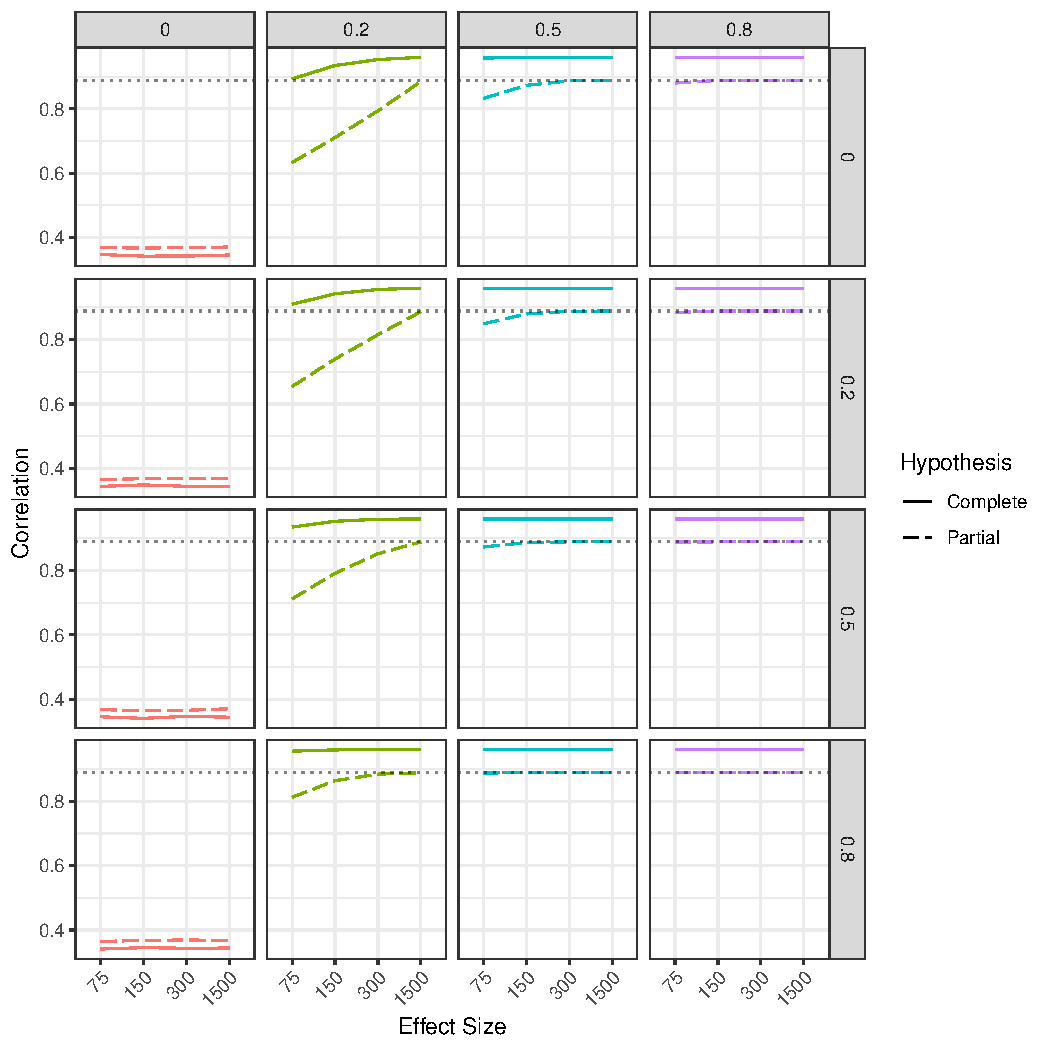
\includegraphics[width=\linewidth]{lineplot.pdf} 
    \caption{The figure shows the comparison of PMPs of a study testing the complete hypothesis ($H_i: \mu_{self} > \mu_{mother} > \mu_{father} > \mu_{teacher}$) against the BES of three studies with partial hypotheses ($H_1: \mu_{self} > \mu_{mother}, H_2: \mu_{mother} > \mu_{father}, H_3: \mu_{father} > \mu_{teacher}$). The complete hypothesis was tested over a sample of size n, while the partial hypotheses each got tested over a sample of n/3. All hypotheses are tested against the unconstrained hypothesis $H_u$. The grey dotted line displays the maximum PMP that the BES can reach due to the limit that the $BF_{1u}$ can reach.}
    \label{fig:lineplot} % This label allows you to refer to the figure
\end{figure}
Overall, Figure \ref{fig:lineplot} indicates that Bayesian Evidence Synthesis is an appropriate way to aggregate evidence, in the case where only partial data sources, that test parts of an overarching hypothesis, are available. In the case of no effect, as can be seen in column one, the BES posterior model probabilities do find slightly more support for $H_1$ than the $PMP_{1u}$, but there still is way larger support for $H_u$. Further, two clear trends can be noted. The effect size plays a big role, large effect sizes ($d \geq 0.5$) reach, or get very close to, the limit of the BES in almost every case. When there is only a small effect ($d = 0.2$), BES still finds good support of the overarching hypothesis, although in small sample sizes it is way smaller than the $PMP_{1u}$ which test the complete hypothesis. When having a large sample ($n_{total} = 1500$), BES also reaches the limit. Higher correlation in the data leads to small improvements in the posterior model probabilities, but compared with the effect of the sample size and effect size, the effect of the correlation is rather small. \\
\begin{figure}[htbp]
    \centering
    \textbf{Comparison of $PMP_{1u}$ and BES for effect size $d = 0.2$ and correlation $\rho = 0.2$} 
    \vspace{0.5em}
    \subfloat[$PMP_{1u}$ of hypothesis $H_i: \mu_{self} > \mu_{mother} > \mu_{father} > \mu_{teacher}$.]{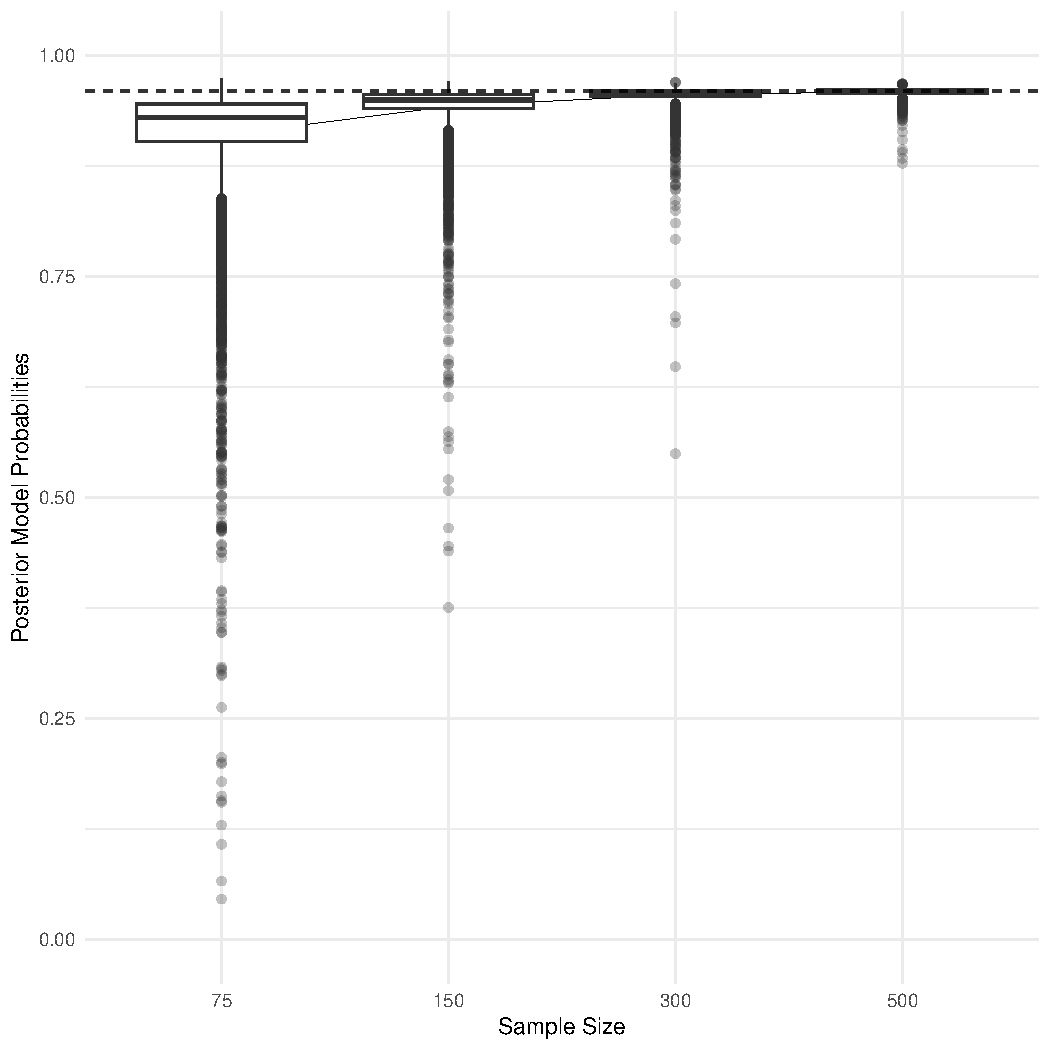
\includegraphics[width=0.45\textwidth]{boxplot_comp.pdf}
    \label{subfig:box_comp}}
    \hfill
    \subfloat[Aggregated BES over three studies with hypotheses $H_1: \mu_{self} > \mu_{mother}; H_2: \mu_{mother} > \mu_{father}; H_3: \mu_{father} > \mu_{teacher}$.]{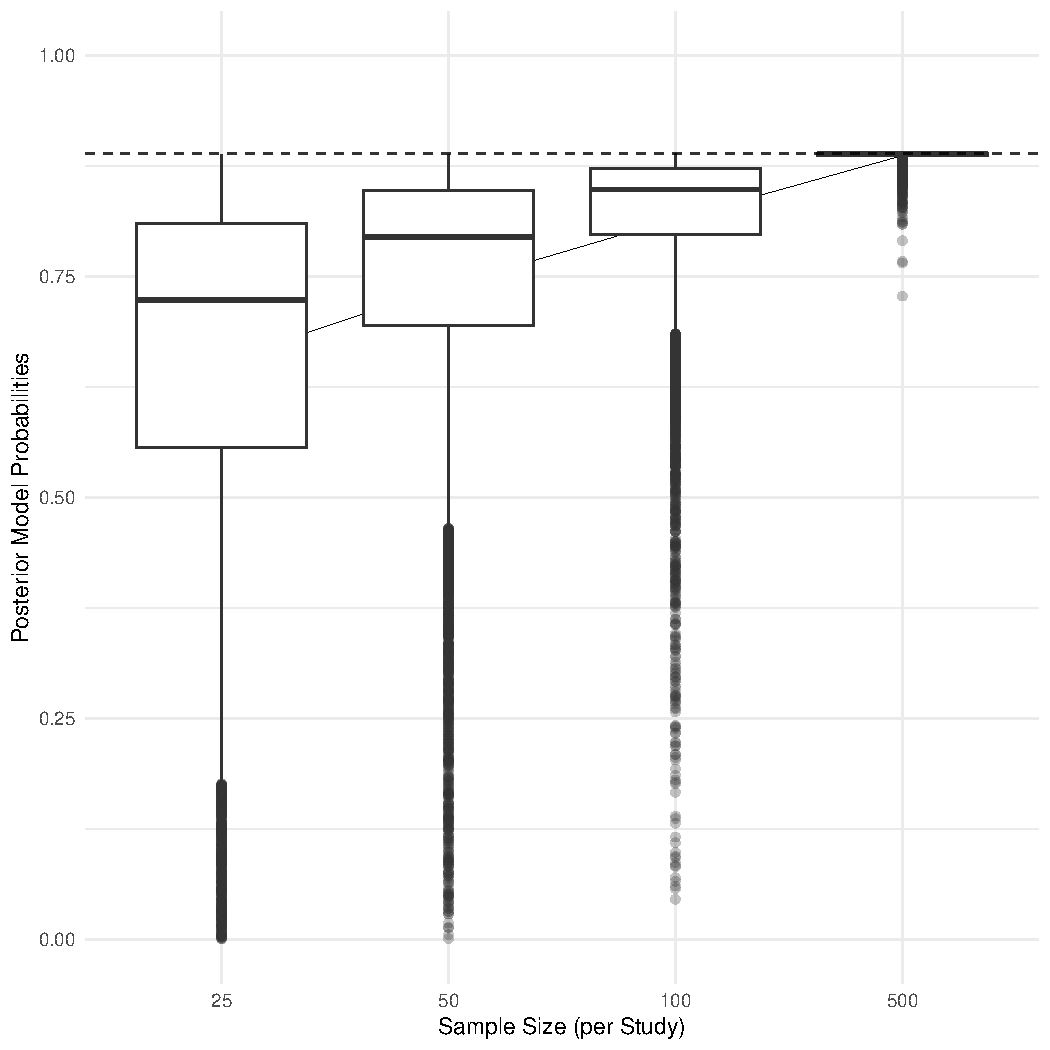
\includegraphics[width=0.45\textwidth]{boxplot_part.pdf}
    \label{subfig:box_part}}
    \caption{The boxplots show the result of the simulations for effect size $d = 0.2$ and correlation $\rho = 0.2$, over 10k iterations. The full black line represents the mean value of the posterior model probability and the dashed black line shows the limit of the $PMP_{1u}$ in Figure \ref{subfig:box_comp} and the limit of the BES in Figure \ref{subfig:box_part}.}
    \label{fig:boxplots}
\end{figure}
Figure \ref{fig:boxplots} is picked out as an interesting case to look at the results in more detail. The boxplots show the results of the simulation over 10k iterations, for effect size $d = 0.2$ and correlation $\rho = 0.2$. Figure \ref{subfig:box_part} shows that there is a higher variability in the results of the BES, compared to testing the complete hypothesis in Figure \ref{subfig:box_comp}. An increasing sample size leads to a steady reduction in the variability, but BES leads to more strong outliers. Overall, the results indicate that Bayesian Evidence Synthesis is an appropriate method to combine the evidence of partial hypotheses, to test an overarching common theory. The BES posterior model probabilities do show a larger variability and more outlier, but all in all, BES produces stable results in these simulation cases. \\
\begin{figure}[htbp]
    \centering
    \textbf{Mean Average Percentage Error over 10k simulations} 
    \vspace{0.5em}
    \subfloat[MAPE over different effect sizes (x-axis) and correlations (y-axis).]{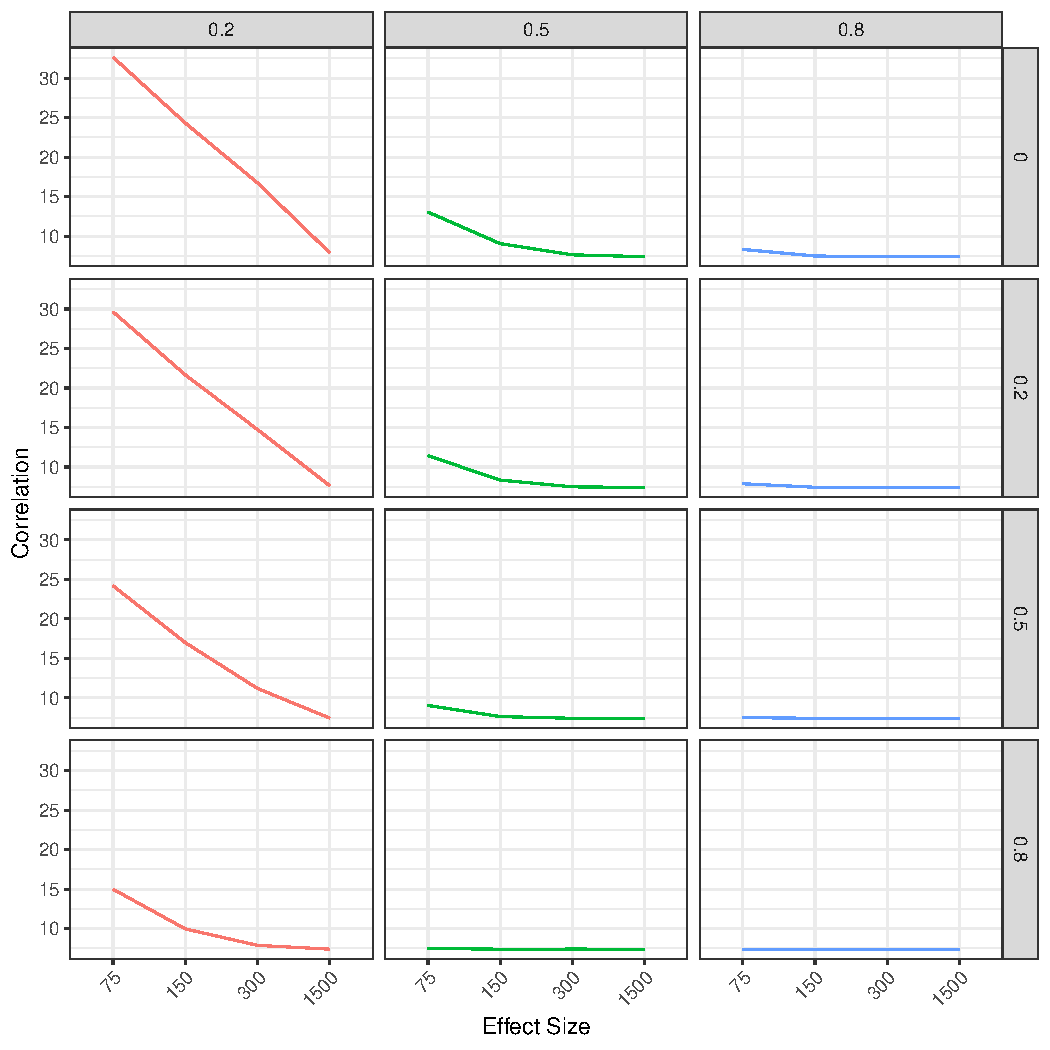
\includegraphics[width=0.45\textwidth]{lineplot_error.pdf}
    \label{subfig:line_MAPE}}
    \hfill
    \subfloat[Boxplot of MAPE for effect size $d = 0.2$ and correlation $\rho = 0.2$.]{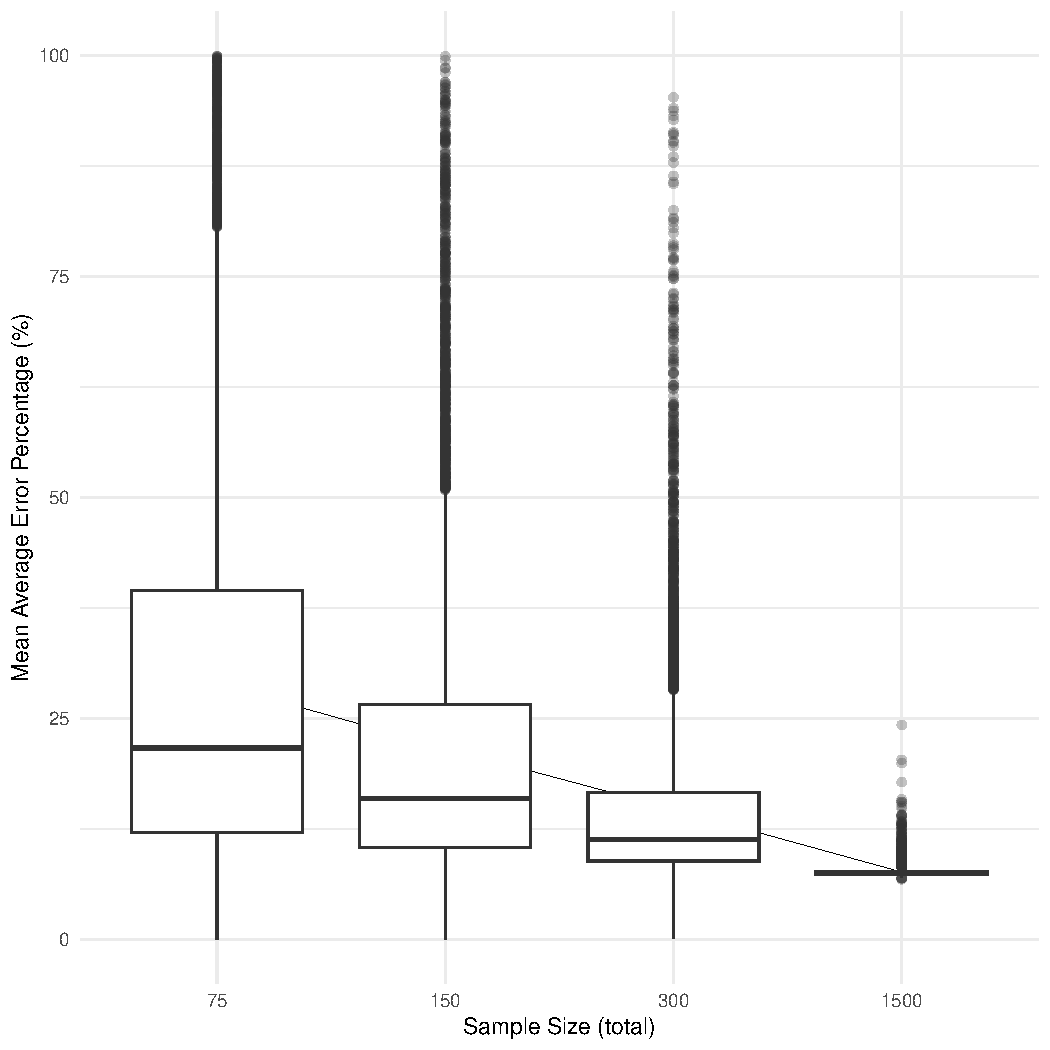
\includegraphics[width=0.45\textwidth]{boxplot_error.pdf}
    \label{subfig:box_MAPE}}
    \caption{The plots show an overview of the MAPE (Figure \ref{subfig:line_MAPE}) and the MAPE for effect size $d = 0.2$ and correlation $\rho = 0.2$ (Figure \ref{subfig:box_MAPE}) over 10k simulations.}
    \label{fig:MAPE}
\end{figure}
Lastly, the Mean Average Percentage Error (MAPE) is shown in Figure \ref{fig:MAPE}. The MAPE is a measure of accuracy and is calculated with the following equation:
\begin{equation}
    MAPE = 100*\frac{1}{n}*\sum_{i=1}^{n}*\left| \frac{PMP_{1u_i} - BES_i}{PMP_{1u_i}} \right|
\end{equation}
\citep{kim_new_2016}. \\
Figure \ref{subfig:line_MAPE} shows that especially with a small effect size ($d = 0.2$), the MAPE tends to be large with up to around 33\%. Increasing the sample size, or with a higher effect size, the MAPE reduces heavily down to about 7\%. High correlation within the data also leads to a small reduction of the MAPE. Figure \ref{subfig:box_MAPE} shows a boxplot of the MAPE for effect size $d = 0.2$ and correlation $\rho = 0.2$. It is clear that increasing sample size leads to a reduction in the variability of the results. While a sample size of 25 observations per study still leads to a large whisker which reaches around 80\%, already increasing the sample size to 50 observations per study reduces the variability largely. While there are strong outliers, the large majority of results are stable. Again, these results indicate that Bayesian Evidence Synthesis is a feasible method to combine the evidence of multiple studies that test partial hypotheses of one overarching theory.

\section{Conclusion}
This report investigated the question, if the synthesis of BFs from studies that evaluate only parts of the overarching hypothesis is a good measure for joint support for the overarching hypothesis. To answer this question, a simulation study was conducted, which was oriented on \citet{kevenaar_bayesian_2021} application of the BES in this way. The simulation conducted BES for studies of varying sample sizes, effect sizes and correlations in the data, but was limited to only testing true hypotheses with the same complexity against the unconstrained hypothesis. The resulting BES were compared with the posterior model probabilities of the overarching hypothesis $H_i: \mu_{self} > \mu_{mother} > \mu_{father} > \mu_{teacher}$, which was tested on a sample of the same size as the combined studies together.\\
Results show that, in this case, Bayesian Evidence Synthesis is an appropriate method to aggregate evidence. While there still is a rather large difference in posterior model probabilities between testing the complete hypothesis and doing BES when the sample size and the effect size are low, BES still finds correct support for the overarching hypothesis. Increasing sample size, or if the effect in the population is of a medium or large size, BES quickly reaches it's limiting value which is effected by the complexity of the hypotheses in each aggregated study. A further measure to compare the results was the Mean Average Percentage Error. The MAPE confirmed the results again. While the error gets as high as about 33\% when the effect and sample sizes are low, increasing the sample size, or a medium to high effect size in the population reduces the error to around 7\%. \\
While these results indicate that BES can be used to aggregate evidence of multiple partial studies to test an overarching hypothesis, there are still multiple aspects that need to be explored to reliably use this method in applied research in the future. One of these aspects is to explore how BES behaves when only parts of the overarching hypothesis is true. An easy first extension to this work could be to switch two of the parameters in the hypothesis, for example to
\begin{equation*}
    H_i: \mu_{self} > \mu_{father} > \mu_{mother} > \mu_{teacher}.
\end{equation*}
This new setup could give new insights in the behaviour of Bayesian Evidence Synthesis. \\
As already mentioned, it is known that the complexity of a hypothesis influences the BF. This relationship should be further explored. In the presented scenario, the complexity of $H_i$ was 24, while the complexity that the BES could reach was only 8. This resulted in different maximal values for the posterior model probabilities. This effect needs to be further investigated. Discussions here could be about scaling BES for the complexities of the partial hypotheses, in comparison to the overarching hypothesis. Another way to investigate the influence of complexity could be to vary the complexity of a hypothesis without changing the other parameters. But this is a challenging task, as it probably needs a more complex study setup with a different effect size measure. Lastly, in this study, the partial hypotheses were chosen in a way that the range of the complete hypothesis was covered with the least amount of information possible. Further research should investigate how BES behaves when the partial hypotheses overlap to a larger extent. 

\section*{Supplementary Material}
\label{sec:supplementary}
All scripts, data and figures are available in the supplementary material on GitHub: \url{https://github.com/flo1met/Internship_BES/}.

\section*{AI Statement}
During the internship and while writing this report, generative AI models (ChatGPT, Grammarly) were solely used for stylistic and grammatical improvements on the text and for assistance during coding.


\newpage

\bibliographystyle{apacite}
\bibliography{bibliography}




\end{document}